
\section{Introduction}
\label{sec:introduction}
%%% General intro
\IEEEPARstart{T}{here} is a growing demand for ubiquitous AI sensor analytics. Industry 4.0 and smart city infrastructure leverage AI solutions to increase productivity and adaptability\cite{lom2016industry}. These solutions are powered by advances in ML, compute engines, and big data. Hence, improvements of these should be considered for research, as they are the machinery of the future.

Convolutional neural networks (CNNs) represent the essential building blocks in 2D pattern analytics. Sensor-based applications such as mechanical fault diagnosis\cite{li2019sensor,dong2018rolling}, structural health monitoring\cite{nagayama2007structural}, human activity recognition (HAR) \cite{wang2019deep}, hazardous gas detection\cite{kim2017hazardous} have been powered by CNN models in industry and academia. CNN-based models, as one of the main types of artificial neural networks (ANNs), have been widely used in sensor analytics with automatic learning from sensor data \cite{ince2016real, janssens2016convolutional, abdeljaber2017real, guo2016hierarchical}. In this context, CNN models are applied for automatic feature learning, usually, from 1D time series as well as for 2D time-frequency spectrograms. CNN models provide advantages such as local dependency, scale invariance, and noise resilience in analytics\cite{du2014leveraging}. However, these models are computationally intensive and power-hungry. This is particularly challenging for low-power embedded applications in the field of Internet-of-Things (IoT).

For ML inference, dedicated hardware architectures are typically used to enhance compute performance and power efficiency. In terms of computational throughput, graphics processing units (GPUs) offer the highest performance; in terms of power efficiency, ASIC and FPGA solutions are more energy efficient \cite{nurvitadhi2017can}. As a result, numerous commercial ASIC and FPGA accelerators have been proposed, targeting both high performance computing (HPC) for data-centers and embedded systems applications.

However, most FPGA accelerators have been implemented to target mid- to high-range FPGAs for computationally intensive CNN models such as AlexNet, VGG-16, and ResNet-18. The main drawbacks of these implementations are power supply demands, physical dimensions, heat sink requirements, air cooling, and high price. In some cases, these implementations are not feasible for ubiquitous low-power/resource-constrained applications.

To reduce the compute hardware for CNN inference there are two types of research \cite{wu2021low}: the first one is deep compression including weight pruning, weight quantization, and compression storage \cite{han2015deep,han2015learning}; the second type of research corresponds to a more efficient data representation, also known as custom quantization for dedicated hardware implementation. In this group, hardware implementations with customized 8-bit floating-point computation have been proposed \cite{mei2017200mhz, wu2021low, lian2019high}. However, these architectures are inadequate for embedded applications, the target devices are high-end FPGA and PCIe devices.

Reducing the compute hardware with more aggressive quantization such as binary \cite{courbariaux2015binaryconnect}, ternary \cite{lin2015neural}, and mixed precision (2-bit activations and ternary weights) \cite{colangelo2018exploration} typically incur significant accuracy degradation for very low precisions, especially for complex problems\cite{faraone2019addnet}.

In this paper, we present the Hybrid-Float6 quantization and its dedicated hardware design. In this concept, feature maps are represented by standard 32-bit FP and trainable parameters by 6-bit FP. To preserve accuracy, we introduce a quantization-aware training (QAT) method. To preserve model accuracy, we present a quantization-aware training method, which in some cases improves model performance. For ML compatibility/portability, the 6-bit FP is wrapped into the standard FP representation. The dedicated hardware design extracts the 6-bit format automatically and performs the computation. We propose a parameterized tensor processor implementing a pipelined vector dot-product with HF6. The 6-bit FP representation uses 4-bit exponent and 1-bit mantissa. This approach enables an optimized MAC design by reducing the mantissa multiplication to a mux-adder operation. We leverage the intrinsic error tolerance of ANN to further reduce the hardware design with approximation. This approach reduces latency, resource utilization, and power dissipation. The embedded hardware/software architecture is integrated with TensorFlow Lite using delegate interface to accelerate \emph{Conv2D} tensor operations. We evaluate the applicability of our approach with a CNN-regression model and hardware design exploration for sensor analytics of SHM for anomaly localization. The embedded hardware/software framework is demonstrated on XC7Z007S as the smallest and most inexpensive Zynq SoC device, see \Fig{fig:workflow}. To the best of our knowledge, this is the first research addressing 6-bit floating-point quantization on CNN models and its dedicated hardware design.

\begin{figure}[t!]
	\centering
	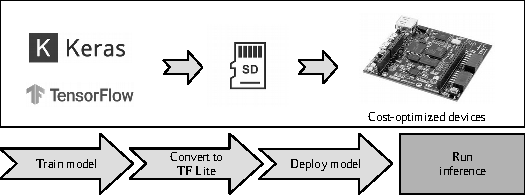
\includegraphics[width=0.5\textwidth]{../figures/workflow.pdf}
	\caption{The workflow of our approach on embedded FPGAs.}
	\label{fig:workflow}
\end{figure}

Our main contributions are as follows:
\begin{enumerate}
	\item
	
	We present the Hybrid-Float6 quantization and its dedicated hardware design. We propose an optimized hardware MAC by reducing the mantissa multiplication to a mux-adder operation. We exploit the intrinsic error tolerance of ANN to further reduce the hardware design with approximation. To preserve model accuracy, we present a quantization-aware training method, which in some cases improves accuracy.
	
	\item We develop a custom hardware/software co-design framework for sensor analytics applications on low-power embedded FPGAs. This architecture integrates TensorFlow Lite.
	\item We present a customizable tensor processor as a dedicated hardware for HF6. This design computes \emph{Conv2D} tensor operations employing a pipelined vector dot-product with parametrized on-chip memory utilization. The compute engine can be implemented with standard floating-point (with FP Xilinx LogiCORE IPs) and HF6.
	\item We demonstrate the potential of our approach with a CNN-regression model for anomaly localization in SHM. We address a hardware design exploration. We evaluate inference accuracy, compute performance, hardware resource utilization, and energy consumption.
\end{enumerate}

The rest of the paper is organized as follows. Section~\ref{sec:related_work} covers the related work; Section~\ref{sec:background} introduces the background for \emph{Conv2D} tensor operation and floating-point number representation; Section~\ref{sec:system_design} describes the system design of the hardware/software architecture and the quantized aware training method; Section~\ref{sec:experimental_results} presents the experimental results thorough a design exploration flow; Section~\ref{sec:conclusions} concludes the paper.

This work is available to the community as an open-source project at https://github.com/YaribNevarez/tensorflow-lite-fpga-delegate.git.